\documentclass{tufte-handout}

\title{One-Way ANOVA with Independent Measures}

%\author[The Tufte-LaTeX Developers]{The Tufte-\LaTeX\ Developers}

\date{} % without \date command, current date is supplied


\usepackage{graphicx} % allow embedded images
  \setkeys{Gin}{width=\linewidth,totalheight=\textheight,keepaspectratio}
  \graphicspath{{graphics/}} % set of paths to search for images
\usepackage{amsmath}  % extended mathematics
\usepackage{booktabs} % book-quality tables
\usepackage{units}    % non-stacked fractions and better unit spacing
\usepackage{multicol} % multiple column layout facilities
\usepackage{lipsum}   % filler text
\usepackage{fancyvrb} % extended verbatim environments
  \fvset{fontsize=\normalsize}% default font size for fancy-verbatim environments

\usepackage{pgfplots}
\pgfplotsset{compat=1.12}

% Standardize command font styles and environments
\newcommand{\doccmd}[1]{\texttt{\textbackslash#1}}% command name -- adds backslash automatically
\newcommand{\docopt}[1]{\ensuremath{\langle}\textrm{\textit{#1}}\ensuremath{\rangle}}% optional command argument
\newcommand{\docarg}[1]{\textrm{\textit{#1}}}% (required) command argument
\newcommand{\docenv}[1]{\textsf{#1}}% environment name
\newcommand{\docpkg}[1]{\texttt{#1}}% package name
\newcommand{\doccls}[1]{\texttt{#1}}% document class name
\newcommand{\docclsopt}[1]{\texttt{#1}}% document class option name
\newenvironment{docspec}{\begin{quote}\noindent}{\end{quote}}% command specification environment


\begin{document}

\maketitle% this prints the handout title, author, and date


%\printclassoptions


\begin{marginfigure}[20pt]
  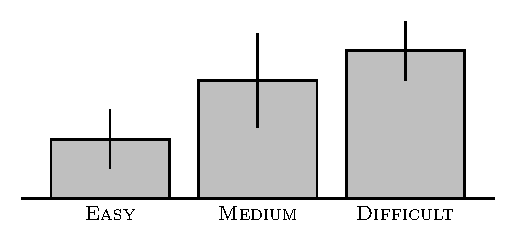
\includegraphics[width=\linewidth]{images/anova_data_one-way}%
  \label{fig:fullfig}%
  \setfloatalignment{t}
  \caption{Data from $k=3$ groups.}
\end{marginfigure}

\begin{marginfigure}[10pt]
  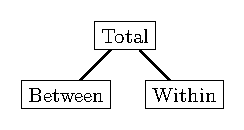
\includegraphics[width=\linewidth]{images/anova_partition_one_way_indep}%
  \label{fig:fullfig}%
  \setfloatalignment{t}
  \caption{Partitioning the Sum of Squares for the One-Way ANOVA with Independent Measures}
\end{marginfigure}

\begin{marginfigure}[10pt]
  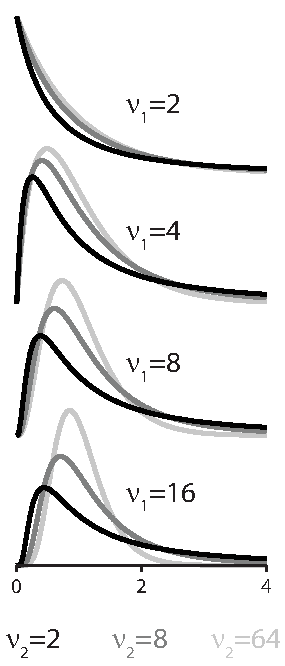
\includegraphics[width=\linewidth]{images/handout4_fpdf}%
  \label{fig:fullfig}%
  \setfloatalignment{t}
  \caption{F-distributions illustrating how the shape varies with different combinations of $\nu_1$ and $nu_2$. Note that we always have $F \geq 0$, and that $F=0$ is the mode when $\nu_1\leq 2$}
\end{marginfigure}


Suppose we wish to determine whether a set of sample means ($\bar{X}_1,\bar{X}_2,\cdots$) show a statistically significant difference. Here, rather than the t-tests that compare two-samples, we can use Analysis of Variance (ANOVA). Like the t-test, the test statistic for ANOVA is a ratio that quantifies differences between means in the numerator and variability within groups in the denominator. However, since ANOVA considers more than two groups we can't just take a simple difference in the numerator, instead we use the variability between groups. For the ANOVA this test statistic is called $F$, and under the null hypothesis $F$ follows an F-distribution. Just like the t-distribution, the shape of the F-distribution depends on the "degrees of freedom." In this case we will need to keep track of both the degrees of freedom for the numerator and degrees of freedom for the denominator, sometimes denoted $\nu_1$ and $\nu_2$. Here is the setup for a one-way ANOVA with independent measures from $k$ groups:

\begin{equation*}
F = \frac{SS_{\text{between groups}}/df_{\text{between groups}}}{SS_{\text{within groups}}/df_{\text{within groups}}}
\end{equation*}

\begin{align*}
&SS_{\text{between groups}}=\sum_{\text{groups}} n_i(\bar{X}_i-\bar{X}_{\text{All}})^2 & &df_{\text{between groups}}=k-1\\
&SS_{\text{within groups}}     =\sum_{\text{groups}} \sum_{\text{scores}} (X-\bar{X}_i)^2 & &df_{\text{within groups}}=N-k
\end{align*}

where the grand mean $\bar{X}_{All}$  is the mean of all scores (no matter which group) and $N$ is the total number of samples (no matter which group)
\begin{equation*}
N=n_1+n_2+\cdots+n_k.
\end{equation*}

One of the key ideas in ANOVA is that variability can be "partitioned" into different sources. It turns out that the different sums of squares and the degrees of freedom are related to each other, and you can often simplify the calculations by thinking about these relationships.
\begin{align*}
&SS_{\text{total}}=\sum (X-\bar{X}_{\text{All}})^2\\
&SS_{\text{total}}=SS_{\text{between groups}} + SS_{\text{within groups}}\\
&df_{\text{total}}=df_{\text{between groups}} + df_{\text{within groups}}=N-1
\end{align*}

Finally, just like the previous hypothesis tests, we would like to quantify effect size. For the ANOVA effect size is determined by "Variance Accounted For", which for independent measures, is 

\begin{equation*}
\eta^2 = \frac{SS_{\text{between groups}}}{SS_{\text{total}}}
\end{equation*}

\pagebreak
\section{Example}

\begin{fullwidth}
Suppose you collect data using a post-test only design with 15 participants in three different groups, and observe the data below. What is the value for the test statistic $F$?

\begin{table}
  \centering
  \fontfamily{ppl}\selectfont
  \begin{tabular}{rccc}
    \toprule
    & Group 1 & Group 2 & Group 3\\
    \midrule
&4&	0&	1\\
&3&	1&	2\\
&6&	3&	2\\
&3&	1&	0\\
&4&	0&	0\\
\midrule
$\bar{X}=$&&&\\
$SS=$&&&\\
    \bottomrule
  \end{tabular}
  \label{tab:normaltab}
  %\zsavepos{pos:normaltab}
\end{table}

\vspace{4.5 in}

\begin{table}
  \centering
  \fontfamily{ppl}\selectfont
  \begin{tabular}{lllll}
    \toprule
    Source & \qquad SS & \qquad df & \qquad MS & \qquad F \\
    \midrule
    Between Groups & & & & \\
    Within Groups & & & & \\
    Total & & & & \\
    \bottomrule
  \end{tabular}
  \label{tab:normaltab}
  %\zsavepos{pos:normaltab}
\end{table}
\end{fullwidth}

\pagebreak
\section{Solution}

\begin{fullwidth}
\begin{table}
  \centering
  \fontfamily{ppl}\selectfont
  \begin{tabular}{rccc}
    \toprule
    & Group 1 & Group 2 & Group 3\\
    \midrule
&4&	0&	1\\
&3&	1&	2\\
&6&	3&	2\\
&3&	1&	0\\
&4&	0&	0\\
\midrule
$\bar{X}=$&4&1&1\\
$SS=$&6&6&4\\
    \bottomrule
  \end{tabular}
  \label{tab:normaltab}
  %\zsavepos{pos:normaltab}
\end{table}
\vspace{20pt}
Based on the data we know $k=3$, and $n_1=n_2=n_3=5$. Let's start by figuring out $SS_{\text{between groups}}$

\begin{equation*}
SS_{\text{between groups}}=\sum_{\text{groups}} n_i(\bar{X}_i-\bar{X}_{\text{All}})^2
\end{equation*}

After calculating the group means (above) we only need the grand mean...

\begin{equation*}
\bar{X}_{\text{All}}=(4+3+6+\cdots)/15=2
\end{equation*}

Now we can fill in

\begin{align*}
&SS_{\text{between groups}}=\sum_{\text{groups}} n_i(\bar{X}_i-\bar{X}_{\text{All}})^2 = 5(4-2)^2+5(1-2)^2+5(1-2)^2=30\\
&df_{\text{between groups}} = k-1 = 3-1=2
\end{align*}

Now let's figure out $SS_{\text{within groups}}$

\begin{align*}
&SS_{\text{within groups}}     =\sum_{\text{groups}} \sum_{\text{scores}} (X-\bar{X}_i)^2 = \sum_{\text{groups}} SS_i = 6+6+4=16\\
&df_{\text{within groups}}=N-k=15-3=12
\end{align*}

Plugging these numbers into the equation for $F$ and using the partitioning to calculate the totals we can fill in the table

\begin{table}
  \centering
  \fontfamily{ppl}\selectfont
  \begin{tabular}{lrrrr}
    \toprule
    Source &  SS &  df & MS &  F \\
    \midrule
    Between Groups & 30 & 2 & 15 & F=11.25 \\
    Within Groups & 16& 12&1.33 & \\
    Total & 46& 14& & \\
    \bottomrule
  \end{tabular}
  \label{tab:normaltab}
  %\zsavepos{pos:normaltab}
\end{table}

\section{Further Questions}
Is this F-ratio statistically significant? What is the effect size?

\end{fullwidth}

\end{document}
